\section{Hashfunktionen}

\begin{frame}
	\frametitle{Was sie tun}
	Eigenschaften
	\begin{columns}
	\column{6cm}
		\begin{itemize}
			\item Surjektiv \begin{small}(Eindeutige Abbildung)\end{small}
			\item Kollisionsfrei
			\item Lawineneffekt
		\end{itemize}
	\column{6cm}
		\begin{center}
			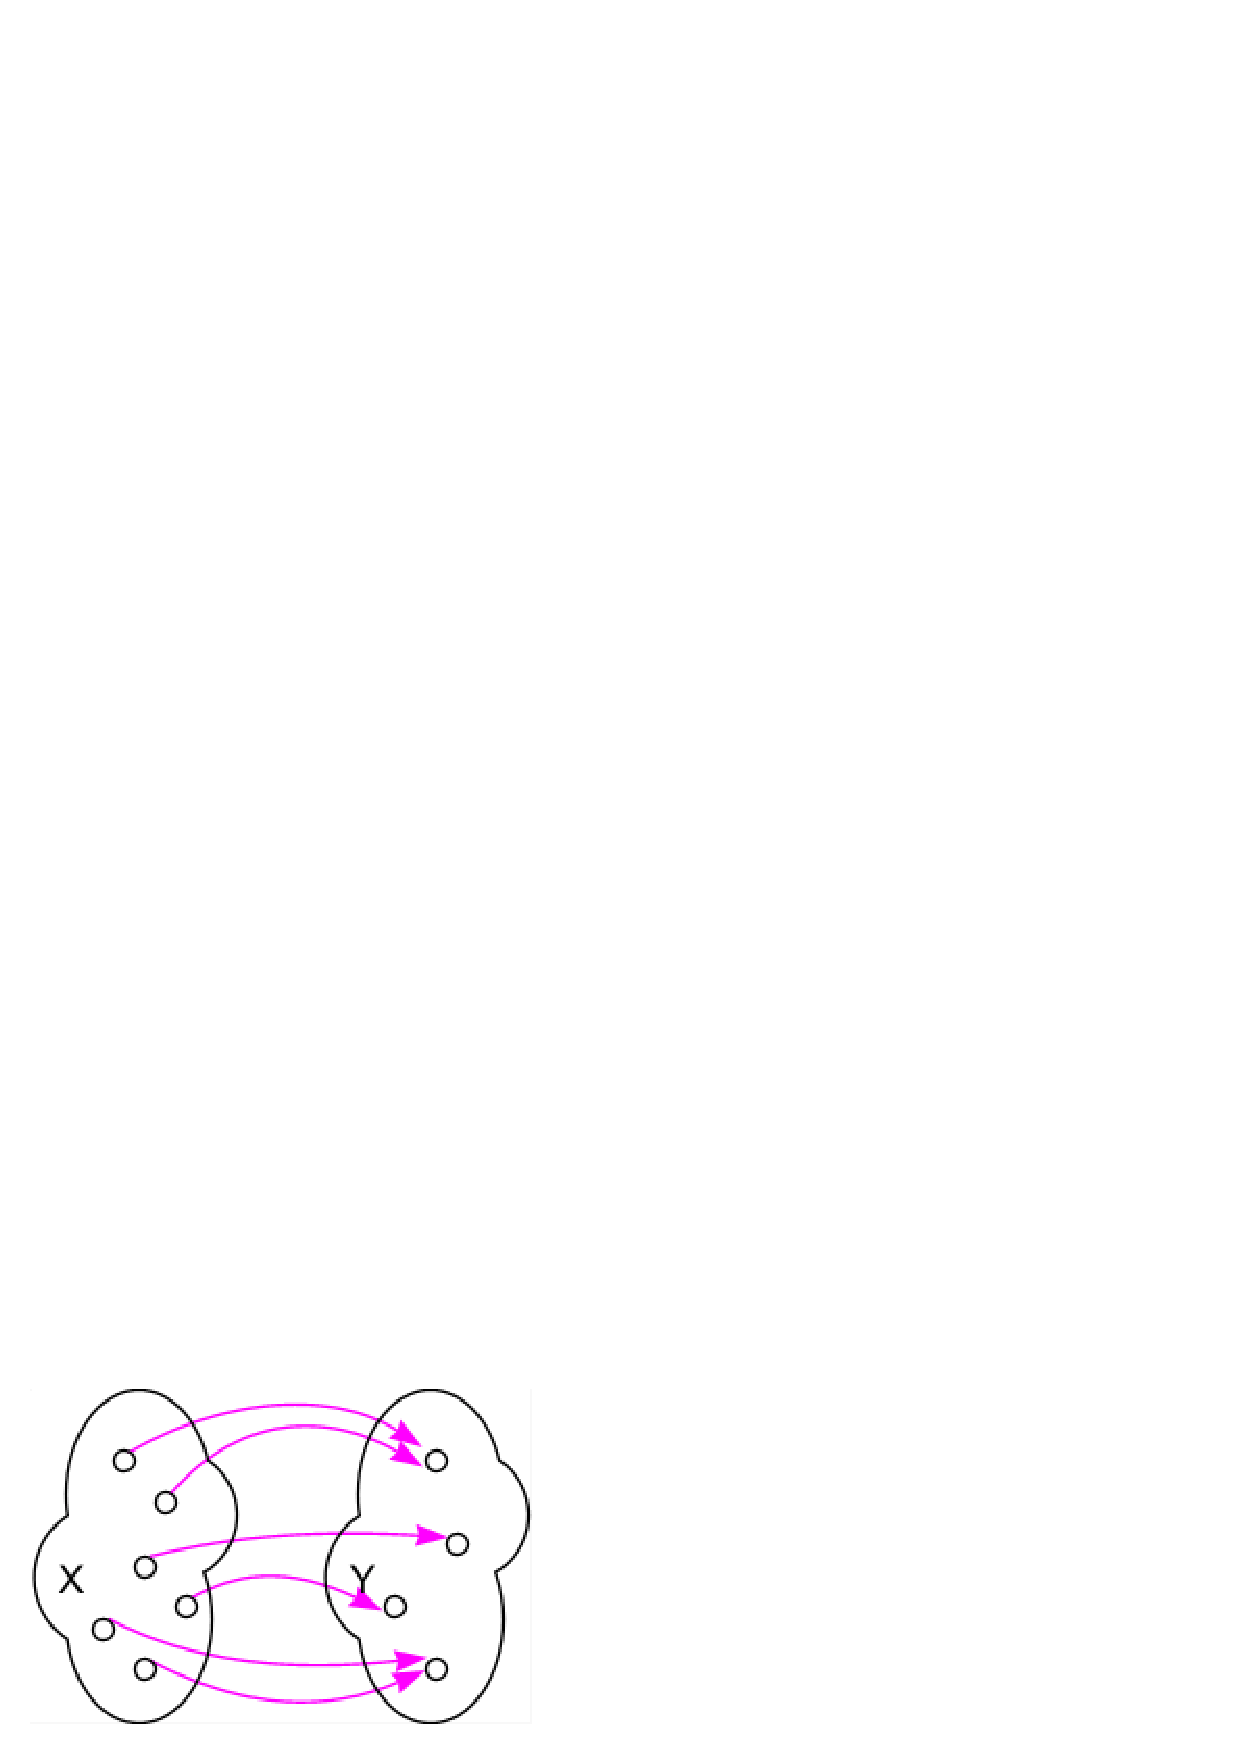
\includegraphics[width=4.8cm,height=3.2cm]{surjektiv}
		\end{center}
	\end{columns}
\end{frame}

\begin{frame}
	\frametitle{Wof"ur?}
	Was bringt's?
	\begin{itemize}
		\item Integrit"at
		\item Authenzit"at \small{(eingeschr"ankt)}
	\end{itemize}

\end{frame}

\begin{frame}
\frametitle{Warum?}
	\begin{columns}
	\column{6cm}
		\begin{itemize}
			\item One-way Eigenschaft
			\item Sinnvoll f"ur gro"se Nachrichten
		\end{itemize}
	\column{6cm}
		\begin{center}
			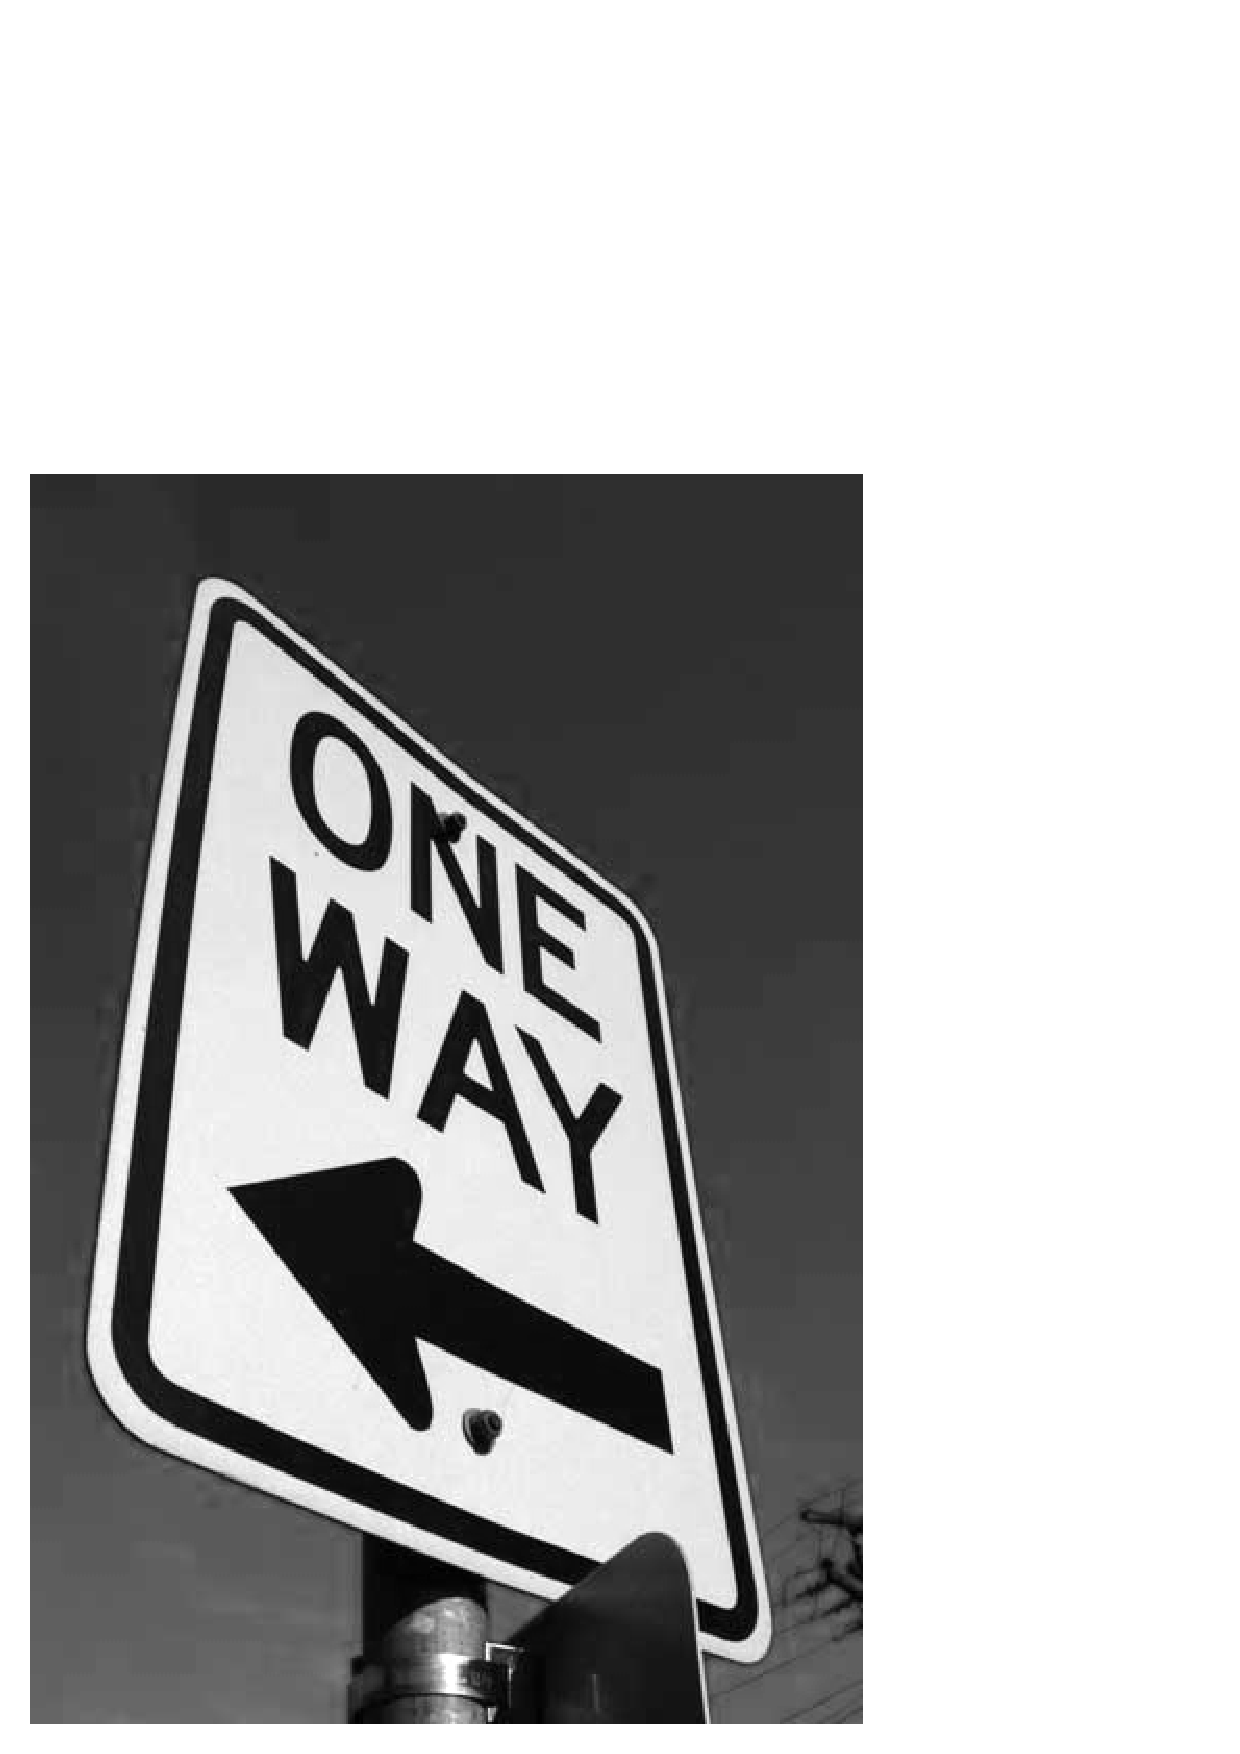
\includegraphics[width=4cm,height=6cm]{oneway}
		\end{center}
	\end{columns}
\end{frame}

\begin{frame}
\frametitle{Wie?}
	Signieren mit gemeinsamen Schl"ussel
	\par
	\begin{center}\large{\texttt{hash ( key | nachricht )}}\end{center}
	\vspace{5mm}
	Speichern von Passw"ortern
	\par
	\begin{center}\large{\texttt{hash ( seed | passwort )}}\end{center}
\end{frame}

\begin{frame}
\frametitle{Angriffe}
	\begin{itemize}
		\item Rainbow Tables (f"ur Passw"orter)
		\item Probieren (z.B. A..z, 0..9)
		\item Reduktion des Problems/Algorithmus
	\end{itemize}
\end{frame}

\begin{frame}
\frametitle{Gegenma"snahmen (1)}
	\large{Immer Salz verwenden!}
\end{frame}

\begin{frame}
\frametitle{Gegenma"snahmen (2)}
	Kaskadieren von Hashfunktionen:
	\par
	\begin{center}\large{\texttt{$hash_1 (msg) \oplus hash_2(msg)$}}\end{center}
	\vspace{5mm}
	\par
	...aber bitte \large{NICHT} so:
	\par
	\begin{center}\large{\texttt{$hash_1 (hash_2(msg))$}}\end{center}
\end{frame}

\end{document}
